La función de Reporte de Estado nos arroja una pantalla como se puede ver en la figura \ref{image:Estado},observamos que nos muestra información reelevante del agente como lo es su comunidad, ip, Sistema Operativo, versión, el numero de interfaces, su ultimo reinicio, su ubicación, el administrador y un pequeño logo del SO del agente.

\FloatBarrier
\begin{figure}[htbp!]
		\centering
	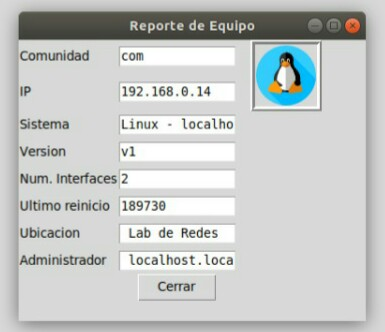
\includegraphics[width=.5 \textwidth]{images/Estado}
		\caption{Ventana emergente de Reporte de Estado, con valores de un agente. }		\label{image:Estado}
\end{figure}
\FloatBarrier


\FloatBarrier
\begin{figure}[htbp!]
		\centering
	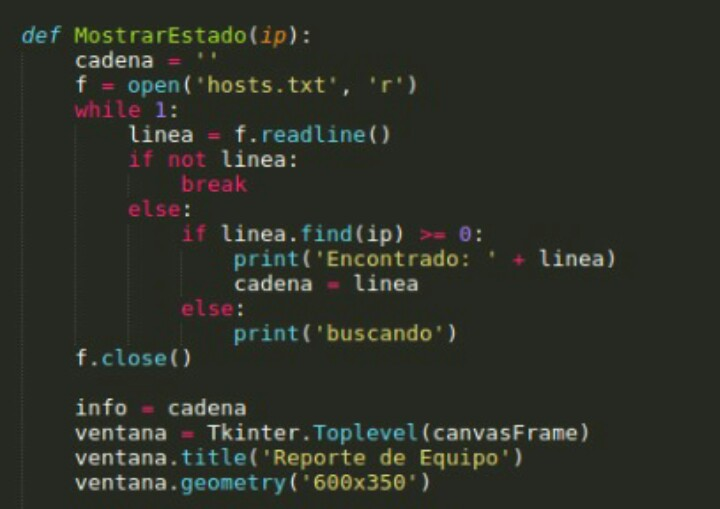
\includegraphics[width=.4 \textwidth]{images/Info}
		\caption{Codigo para generar la ventana. }		\label{image:Info}
\end{figure}
\FloatBarrier

Para consultar dicha información del agente se necesitaron las siguientes consulas SNMP con los OID(unicamente para el sistema, num. de interfacez, último reinicio, ubicación y adminitrador):


	\textbf{S.O -- 1.3.6.1.2.1.1.1.0}


	\textbf{Número de interfaces -- 1.3.6.1.2.1.2.1.0}


	\textbf{último Reinicio -- 1.3.6.1.2.1.1.3.0}


	\textbf{Ubicación -- 1.3.6.1.2.1.1.6.0}


	\textbf{Administrador -- 1.3.6.1.2.1.1.5.0}
	
	
La información faltante se obtuvo del archivo Host.txt  y se extrajo la comunidad, la versión y la IP, como se muestra e la figura  \ref{image:Codigo}

\FloatBarrier
\begin{figure}[htbp!]
		\centering
	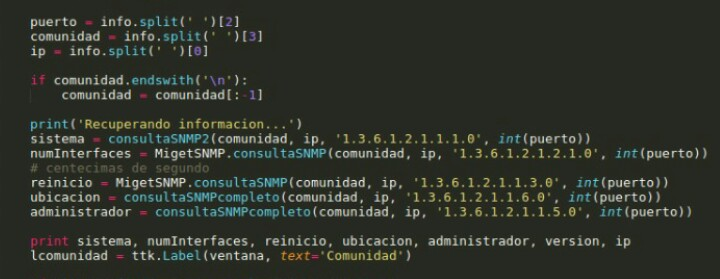
\includegraphics[width=.7 \textwidth]{images/Codigo}
		\caption{Ventana emergente de Reporte de Estado, con valores de un agente. }		\label{image:Codigo}
\end{figure}
\FloatBarrier


finalmente para poder ver el logo del sistema operativo como se muestra en la figura   \ref{image:linux} se implemento el siguiente codigo  figura      \ref{image:Cologo}

\FloatBarrier
\begin{figure}[htbp!]
		\centering
	
\includegraphics[width=.2 \textwidth]{images/linux}
		\caption{Logo del S.O Linux. }		\label{image:linux}
\end{figure}
\FloatBarrier

\FloatBarrier
\begin{figure}[htbp!]
		\centering
	
\includegraphics[width=.2\textwidth]{images/windows}
		\caption{Logo del S.O Windows. }		\label{image:windows}
\end{figure}
\FloatBarrier


\FloatBarrier
\begin{figure}[htbp!]
		\centering
	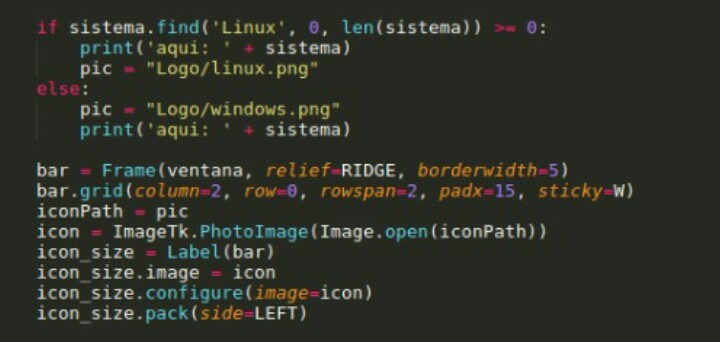
\includegraphics[width=.7\textwidth]{images/Cologo}
		\caption{Implementación del logo del agente, fue necesario importar Image e ImageTK }		\label{image:Cologo}
\end{figure}
\FloatBarrier